\subsection{Система мониторинга как процесс}

Входным объектом существующей в настоящее время системы мониторинга является сам
пациент. На выходе системы врачи выдают медицинское заключение о состоянии
здоровья пациента.

В процессе мониторинга в настоящее время используются всевозможные лабораторные
анализы, а также дневник наблюдения (который ведут родители или опекуны
пациента). В качестве оборудования также используются персональные компьютеры на
которых ведется база данных пациентов (представляет собой файл электронной
таблицы Excel). Следят за процессом мониторинга лица, назначqенные руководством
кардиоцентра и другие государственные служащие. Общая схема процесса мониторинга
изображена на рисунке \ref{ris:before_decomposition}.

\begin{figure}[h]
\center{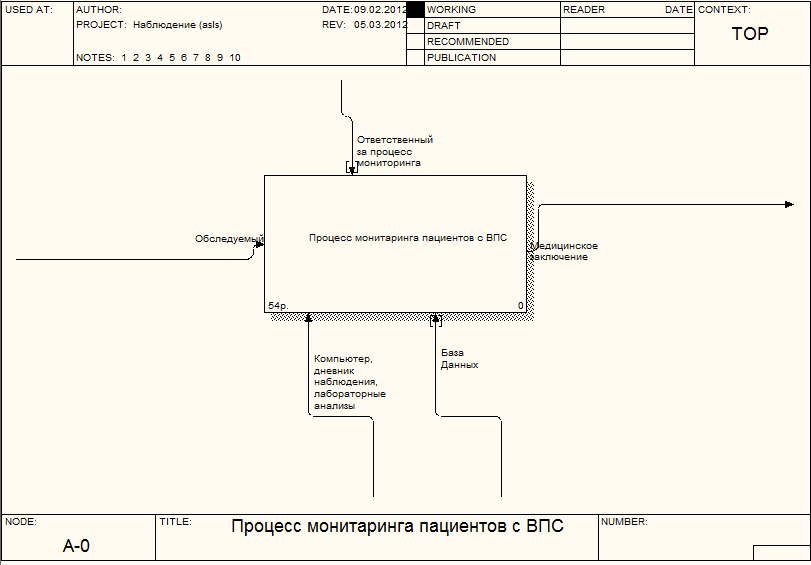
\includegraphics[width=1\linewidth]{before_decomposition.eps}}
\caption{Общая схема процесса мониторинга}
\label{ris:before_decomposition}
\end{figure}

\subsection{Система мониторинга как совокупность процессов}

Как правило процесс мониторинга пациентов с ВПС (как и многие другие виды
лечений) начинается с предварительного приема (рисунок \ref{ris:as_is_general_diagram}). Прием
проводится в учреждении здравохранения по месту жительства - это позволяет к моменту приема
непосредственно в кардиоцентре  иметь некоторую медицинскую информацию
(результаты анализов, самостоятельные наблюдения пациента) и соответственно
разгрузить персонал и оборурдование ККЦ от большой входной нагрузки,
сконцетрировавашись на основной своей деятльности.

\begin{figure}[h]
\center{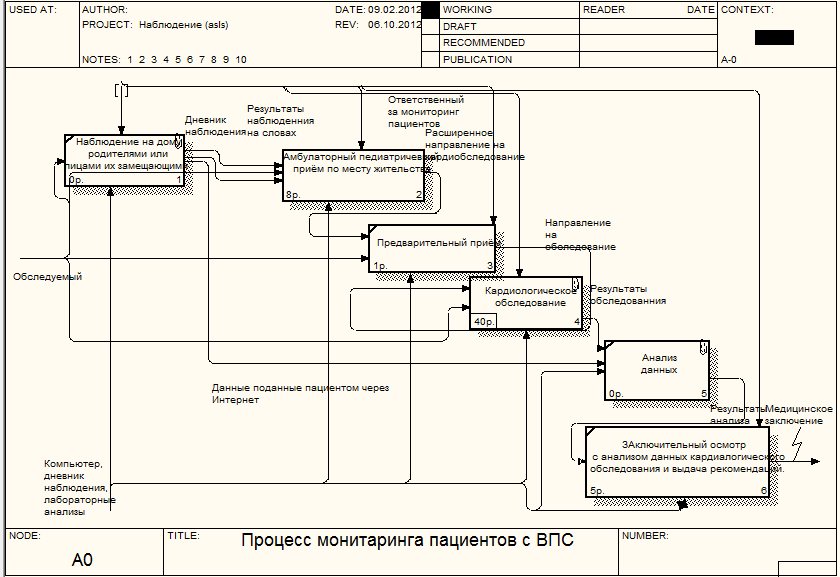
\includegraphics[width=1\linewidth]{as_is_general_diagram.eps}}
\caption{Декомпозиция процесса мониторинга}
\label{ris:as_is_general_diagram}
\end{figure}

Во время врачебного приема родители пациента передают медицинскую информацию
(как правило это результаты наблюдения за его состоянием) словесно, а также  в
виде дневника наблюдения.

\subsection{Амбулаторный педиатрический прием}

Одним из трудоемким для обоих сторон процессов является периодический
амбулаторный прием по месту жительства (рисунок \ref{ris:ambulator_appointment}).

\begin{figure}[h]
\center{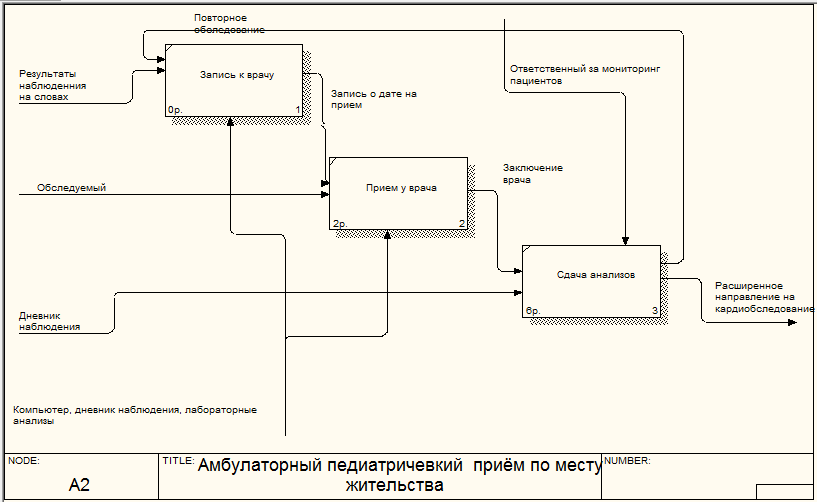
\includegraphics[width=1\linewidth]{ambulator_appointment.eps}}
\caption{Прием у врача}
\label{ris:ambulator_appointment}
\end{figure}

Данный процесс состоит из 3 стадий. Сперва больной записывается на прием к
врачую. Во время записи родители пациента вносят записи о результатах своих
наблюдений. Далее больной приходит на прием к врачу. Врач по итогам осмотра
выдает заключение и направляет пациента на сдачу медицинскиха анализов. На
основаниии анализов либо проводится либо повторное обследование, либо выдается
расширенное направление на кардиобследование.

\subsection{Заключительная стадия мониторинга}

После кардиологического обследования пациента, врачи проводят анализ полученной
медицинской информации. На основании сделанных выводов врачи составляют
медицинское заключение и выдают рекомендации родителям и лечащим врачам. Данная
информация сообщается пациенту на заключительном осмотре.